\documentclass[../Main.tex]{subfiles}
\begin{document}
  \chapter{2024-2025学年微积分（B）（下）期中考试}

  \section{基本计算题(每小题 6 分，共 60 分)}
  \begin{enumerate}
    \item 设$M_{0}(2,-1,1)$，$M_{1}(3,2,-1)$，$M_{2}(1,3,-2)$是空间三点，$\boldsymbol
      {l}$为与向量$2\overrightarrow{M_0M_1}-2\overrightarrow{M_0M_2}$方向相同的单位向量，求以$\boldsymbol
      {l}$，$\overrightarrow{M_0M_1}$为邻边的平行四边形的面积$S$.
      \vspace{10em}

    \item 已知单位向量$\overrightarrow{OA}$与三个坐标轴正向的夹角相等，且夹角的方向余弦为正，点$B$是点$M
      (1,1,-1)$关于点$N(-1,2,1)$的对称点，求$\angle AOB$的角平分线上的单位向量.
      \vspace{10em}

    \item 求二重极限$\lim_{\substack{x\to 0 \\ y\to 0}}\frac{\ln\left(1+2x^{2}+2y^{2}\right)}{\sqrt{x^{2}+y^{2}}\sin\sqrt{x^{2}+y^{2}}}$.
      \vspace{10em}

    \item 将曲线$L:
      \begin{cases}
        z=x^{2}+1, \\
        y=0
      \end{cases}$绕$z$轴旋转一周得到一个旋转曲面$S$，求该旋转曲面$S$与平面$x+y+z
      =1$的交线的参数方程.
      \vspace{12em}

    \item 设函数$f(x,y)=x^{2}(y-3)+(x-1)\arctan\sqrt{\frac{x}{y}}$，求$\left.\mathrm{d}
      f\right|_{(1,3)}$.
      \vspace{12em}

    \item 设$u=f(x,y,z)$有连续的一阶偏导数，$y=y(x)$由方程$\mathrm{e}^{xy}=xy+2$确定，$z
      =z(x)$由方程$\mathrm{e}^{x} = \int_{0}^{x-z}\mathrm{e}^{t^2}\mathrm{d}t$确定，求$\frac{\mathrm{d}u}{\mathrm{d}x}$.
      \vspace{12em}

    \item 计算二次积分$I=\int_{0}^{4}\mathrm{d}x\int_{\sqrt{x}}^{2}\frac{1}{\sqrt{1+y^{3}}}
      \mathrm{d}y$.
      \vspace{12em}

    \item 设函数$z=g\left(\frac{y}{x}\right)+f\left(xy,\frac{x}{y}\right)$，其中$f
      (u,v)$具有二阶连续的偏导数，$g(t)$二阶导数连续，试求$\frac{\partial^{2} z}{\partial
      x \partial y}$.
      \vspace{10em}

    \item 计算二重积分
      \[
        I=\iint\limits_{D}\left(x^{2} y+\left(y^{3}+x\right)\sqrt{x^{2}+y^{2}}\right
        )\mathrm{d}x\mathrm{d}y,
      \]
      其中$D:x^{2}+y^{2}\leq 2x$.
      \vspace{10em}

    \item 计算三重积分$I=\iiint\limits_{V}(y+2z)\mathrm{d}V$，其中$V$由锥面$z=\sqrt{x^{2}+y^{2}}$与$z
      =\sqrt{1-x^{2}-y^{2}}$所围成.
      \vspace{10em}
  \end{enumerate}

  \section{综合题(每小题 8 分，共 40 分)}
  \begin{enumerate}
    \setcounter{enumi}{10}
    \item 设向量$\boldsymbol{a}=(2,-1,1)$，$\boldsymbol{b}=(1,2,3)$，向量$\boldsymbol
      {d}$与向量$\boldsymbol{a}$，$\boldsymbol{b}$均垂直，且与$z$轴夹锐角，求函数$u
      =xy+2y+3zx$在点$M_{0}(1,-2,1)$处沿方向$\boldsymbol{d}$的方向导数.
      \vspace{13em}

    \item 设曲线$\begin{cases}
        x^{2}+y^{2}+z^{2}=6, \\
        x+y+z=0
      \end{cases}$在点$Q(1,1,-2)$处的切线为$l$，曲面$xy+z=0$在点$P_{0}(2,1,-2)$处的切平面为$\pi$，求切线$l$在平面$\pi$上的投影直线的方程.
      \vspace{10em}

    \item 记曲面$z=x^{2}+y^{2}-xy+x+y$在区域$D:x\leq 0,y\leq 0,x+y\geq -3$上的最低点为$Q$，求过点$Q$且与直线$\begin{cases}
        x+2y-z=1, \\
        2x+y-z=0
      \end{cases}$垂直的平面方程.
      \vspace{10em}

    \item 讨论函数$f(x,y)=
      \begin{cases}
        \frac{\sin(xy^{2})}{x^{2}+y^{2}}, & (x,y)\neq(0,0), \\
        0,                                & (x,y)=(0,0)
      \end{cases}$在原点处的连续性、偏导数存在性及可微性.
      \vspace{10em}

    \item 设函数$f(x,y)$在全平面内可微，且满足$x\frac{\partial f}{\partial
      x}+y\frac{\partial f}{\partial y}=0$，证明：

      $\forall\,t\in\mathbf{R}$，$f(tx,ty)=f(x,y)$，即$f(x,y)$恒为常数.
      \vspace{10em}
  \end{enumerate}

  \chapter{2024-2025学年微积分（B）（下）期中考试参考答案}
  \section{基本计算题(每小题 6 分，共 60 分)}
  \begin{enumerate}
    \item \textbf{Solution}. 由题可知$\overrightarrow{M_0M_1}=(1,3,-2)$，$\overrightarrow
      {M_0M_2}=(-1,4,-3)$，

      所以$2\overrightarrow{M_0M_1}-2\overrightarrow{M_0M_2}=(4,-2,2)$，$\boldsymbol
      {l}=\frac{1}{\sqrt{6}}(2,-1,1)$.

      $S=|\boldsymbol{l}\times\overrightarrow{M_0M_1}|=\frac{1}{\sqrt{6}}|(-1,5,7
      )|=\frac{5\sqrt{2}}{2}$.

    \item \textbf{Solution}. 由题可知$\overrightarrow{OA}=\frac{1}{\sqrt{3}}(1,1,
      1)$，$B(-3,3,3)$，$\overrightarrow{OB}=3(-1,1,1)$.

      设$\overrightarrow{OB}$方向上的单位向量为$\boldsymbol{u}$，则$\boldsymbol{u}
      =\frac{1}{\sqrt{3}}(-1,1,1)$.

      故$\angle AOB$的角平分线上的单位向量为$\frac{\overrightarrow{OA}+\boldsymbol{u}}{|\overrightarrow{OA}+\boldsymbol{u}|}
      =\frac{(0,\frac{2}{\sqrt{3}},\frac{2}{\sqrt{3}})}{\frac{2\sqrt{2}}{\sqrt{3}}}
      =\frac{1}{\sqrt{2}}(0,1,1)$.

    \item \textbf{Solution}.
      \[
        \begin{aligned}
          l = \lim_{\substack{x\to 0 \\ y\to 0}}\frac{\ln\left(1+2x^2+2y^2\right)}{\sqrt{x^2+y^2}\sin\sqrt{x^2+y^2}}= & \lim_{\substack{x\to 0 \\ y\to 0}}\frac{2x^2+2y^2}{\sqrt{x^2+y^2}\cdot\sqrt{x^2+y^2}} \\
          =                                                                                                           & \lim_{\substack{x\to 0 \\ y\to 0}}\frac{2(x^2+y^2)}{x^2+y^2}=2.
        \end{aligned}
      \]

    \item \textbf{Solution}. 由题可得$S$的方程为$z=x^{2}+y^{2}+1$，所以交线为$\begin{cases}
        z=x^{2}+y^{2}+1, \\
        x+y+z=1.
      \end{cases}$

      消去$z$得$x^{2}+y^{2}+x+y=0$，即$\left(x+\frac{1}{2}\right)^{2}+\left(y+\frac{1}{2}
      \right)^{2}=\frac{1}{2}$.

      令$\begin{cases}
        x = \frac{\sqrt{2}}{2}\cos \theta-\frac{1}{2}, \\
        y = \frac{\sqrt{2}}{2}\sin \theta-\frac{1}{2}
      \end{cases}(0\leq \theta < 2\pi)$，则$z=1-x-y=2-\frac{\sqrt{2}}{2}(\cos \theta
      +\sin \theta)=2-\sin\left(\theta+\frac{\pi}{4}\right)$.

      因此交线的参数方程为$\begin{cases}
        x = \frac{\sqrt{2}}{2}\cos \theta-\frac{1}{2}, \\
        y = \frac{\sqrt{2}}{2}\sin \theta-\frac{1}{2}, \\
        z = 2-\sin\left(\theta+\frac{\pi}{4}\right)
      \end{cases}(0\leq \theta < 2\pi)$.

    \item \textbf{Solution}. 方程$f(x,y) = x^{2}(y-3)+(x-1)\arctan\sqrt{\frac{x}{y}}$两边全微分，得
      \[
        \begin{aligned}
          \mathrm{d}f = & 2x\mathrm{d}x\cdot (y-3) +x^{2} \mathrm{d}y +\mathrm{d}x\cdot \arctan\sqrt{\frac{x}{y}}+(x-1)\cdot\frac{1}{1+\frac{x}{y}}\cdot \frac{1}{2\sqrt{\frac{x}{y}}}\cdot\left(\frac{y\mathrm{d}x-x\mathrm{d}y}{y^2}\right) \\
          =             & 2x(y-3)\mathrm{d}x +x^{2}\mathrm{d}y+\arctan\sqrt{\frac{x}{y}}\mathrm{d}x+(x-1)\cdot\frac{y\mathrm{d}x-x\mathrm{d}y}{2y^2\sqrt{\frac{x}{y}}\left(1+\frac{x}{y}\right)}.
        \end{aligned}
      \]

      所以$\left.\mathrm{d}f\right|_{(1,3)}=\mathrm{d}y + \arctan\frac{1}{\sqrt{3}}
      \mathrm{d}x = \frac{\pi}{6}\mathrm{d}x + \mathrm{d}y$.

    \item \textbf{Solution}. 令$F(x,y) = \mathrm{e}^{xy}-xy-2$，

      注意到当$xy = 0$时，方程$\mathrm{e}^{xy}= xy+2$不成立，所以$F(x,y)$的定义域为$x
      \neq0,y\neq0$.

      $\frac{\mathrm{d}y}{\mathrm{d}x}=-\frac{F'_{x}}{F'_{y}}=-\frac{y\mathrm{e}^{xy}-y}{x\mathrm{e}^{xy}-x}
      =-\frac{y}{x}$.

      令$G(x,z) = \mathrm{e}^{x} - \int_{0}^{x-z}\mathrm{e}^{t^2}\mathrm{d}t$，

      注意到当$x-z=0$时，方程$\mathrm{e}^{x} = \int_{0}^{x-z}\mathrm{e}^{t^2}\mathrm{d}
      t$不成立，所以$G(x,z)$的定义域为$x\neq z$.

      $\frac{\mathrm{d}z}{\mathrm{d}x}=-\frac{G'_{x}}{G'_{z}}=-\frac{\mathrm{e}^{x}-\mathrm{e}^{(x-z)^2}}{\mathrm{e}^{(x-z)^2}}$.

      所以$\frac{\mathrm{d}u}{\mathrm{d}x}=f'_{1}\cdot 1+f'_{2}\cdot \frac{\mathrm{d}y}{\mathrm{d}x}
      +f'_{3}\cdot \frac{\mathrm{d}z}{\mathrm{d}x}=f'_{1}-f'_{2}\cdot \frac{y}{x}
      +f'_{3}\cdot \frac{\mathrm{e}^{x}-\mathrm{e}^{(x-z)^2}}{\mathrm{e}^{(x-z)^2}}$（$x
      \neq0,y\neq0,x\neq z$）.

    \item \textbf{Solution}. 积分区域$D$如右图所示.交换积分次序得
      \begin{figure}[h] % 图片
        \small \raggedleft
        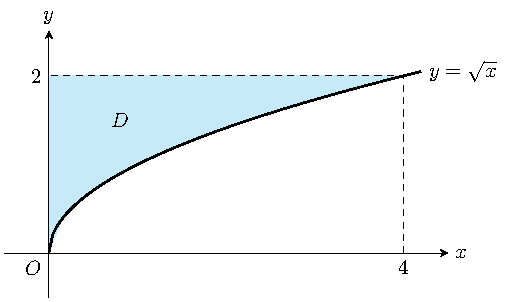
\includegraphics[width=6cm]{2025x-figure.pdf} % 引入图片源
      \end{figure} % 图片结束
      \vspace{-13em}

      $\begin{aligned}
        I = & \int_{0}^{2}\mathrm{d}y\int_{0}^{y^2}\frac{1}{\sqrt{1+y^3}}\mathrm{d}x = \int_{0}^{2}\frac{y^2}{\sqrt{1+y^3}}\mathrm{d}y \\
        =   & \frac{1}{3}\int_{0}^{2}\frac{\mathrm{d}\left(1+y^3\right)}{\sqrt{1+y^3}}                                                 \\
        =   & \left.\frac{2}{3}\sqrt{1+y^3}\right|_{0}^{2}=\frac{2}{3}\left(\sqrt{9}-1\right)=\frac{4}{3}.
      \end{aligned}$

    \item \textbf{Solution}. $\frac{\partial z}{\partial x}= g'\left(\frac{y}{x}\right
      )\cdot\left(-\frac{y}{x^{2}}\right)+f'_{1}\cdot y+f'_{2}\cdot \frac{1}{y}$,

      $\frac{\partial^{2} z}{\partial x \partial y}= \left[-\frac{1}{x^{2}}g'\left
      (\frac{y}{x}\right)-\frac{y}{x^{2}}\cdot\frac{1}{x}g''\left(\frac{y}{x}\right
      )\right]+\left[f'_{1}+y\left(xf''_{11}-\frac{x}{y^{2}}f''_{12}\right)\right
      ]+\left[-\frac{1}{y^{2}}f'_{2}+\frac{1}{y}\left(xf''_{21}-\frac{x}{y^{2}}f''_{22}\right)\right]$.

      由于$f(u,v)$二阶偏导数连续，所以$f''_{12}=f''_{21}$，整理得
      \[
        \frac{\partial^{2} z}{\partial x \partial y}= -\frac{1}{x^{2}}g'\left(\frac{y}{x}
        \right)-\frac{y}{x^{3}}g''\left(\frac{y}{x}\right)+f'_{1}-\frac{1}{y^{2}}
        f'_{2}+xyf''_{11}-\frac{x}{y^{3}}f''_{22}.
      \]

    \item \textbf{Solution}. 积分区域$D$是以点$(1,0)$为圆心，半径$1$的圆盘.

      由于$D$关于$x$轴对称，且$x^{2}y$与$y^{3}\sqrt{x^{2}+y^{2}}$关于$y$均为奇函数，所以
      \[
        \iint\limits_{D}x^{2} y\mathrm{d}x\mathrm{d}y=\iint\limits_{D}y^{3}\sqrt{x^{2}+y^{2}}
        \mathrm{d}x\mathrm{d}y=0.
      \]

      故$I=\iint\limits_{D}x\sqrt{x^{2}+y^{2}}\mathrm{d}x\mathrm{d}y$.

      用极坐标代换，$D$的极坐标方程为$r=2\cos \theta$，其中$-\frac{\pi}{2}\leq \theta
      \leq \frac{\pi}{2}$，所以
      \[
        \begin{aligned}
          I = & \int_{-\frac{\pi}{2}}^{\frac{\pi}{2}}\mathrm{d}\theta\int_{0}^{2\cos\theta}r\cos\theta\cdot r^{2}\mathrm{d}r = 4\int_{-\frac{\pi}{2}}^{\frac{\pi}{2}}\cos^{5}\theta\mathrm{d}\theta \\
          =   & 8\int_{0}^{\frac{\pi}{2}}\cos^{5}\theta\mathrm{d}\theta = 8\cdot\frac{4\cdot2}{5\cdot3}=\frac{64}{15}.
        \end{aligned}
      \]

    \item \textbf{Solution}. 由积分区域$V$的对称性易知$\iiint\limits_{V}y\mathrm{d}
      V=0$，所以
      \[
        I = 2\iiint\limits_{V}z\mathrm{d}V = 2\iint\limits_{D_{xy}}\mathrm{d}x\mathrm{d}
        y\int_{\sqrt{x^{2}+y^{2}}}^{\sqrt{1-x^{2}-y^{2}}}z\mathrm{d}z,
      \]

      其中$D_{xy}$是锥面和半球面的交线在$xOy$平面上的投影区域，即$x^{2}+y^{2}\leq
      \frac{1}{2}$.

      用柱坐标代换，锥面的方程为$z=r$，半球面的方程为$z=\sqrt{1-r^{2}}$，所以
      \[
        \begin{aligned}
          I = & 2\iint\limits_{D_{xy}}\mathrm{d}x\mathrm{d}y\int_{\sqrt{x^2+y^2}}^{\sqrt{1-x^2-y^2}}z\mathrm{d}z                              \\
          =   & 2\int_{0}^{2\pi}\mathrm{d}\theta \int_{0}^{\frac{\sqrt{2}}{2}}r\mathrm{d}r\int_{r}^{\sqrt{1-r^2}}z\mathrm{d}z                 \\
          =   & 2\pi\int_{0}^{\frac{\sqrt{2}}{2}}r(1-r^{2}-r^{2})\mathrm{d}r = \pi(r^{2}-r^{4})\Bigg|_{0}^{\frac{\sqrt{2}}{2}}=\frac{\pi}{4}.
        \end{aligned}
      \]
  \end{enumerate}

  \section{综合题(每小题 8 分，共 40 分)}
  \begin{enumerate}
    \setcounter{enumi}{10}
    \item \textbf{Solution}. $\boldsymbol{a}\times \boldsymbol{b}= (-5,-5,5)$，取$\boldsymbol
      {d}= \frac{1}{\sqrt{3}}(-1,-1,1)$.

      $\nabla u = (y+3z, x+2, 3x)$，所以$\nabla u|_{M_0}= (1,3,3)$.

      $\frac{\partial u}{\partial \boldsymbol{d}}= \nabla u|_{M_0}\cdot \boldsymbol
      {d}= -\frac{1}{\sqrt{3}}-\sqrt{3}+\sqrt{3}= -\frac{\sqrt{3}}{3}$.

    \item \textbf{Solution}. 设$l$的一个方向向量为$\boldsymbol{l}$，$\pi$的一个法向量为$\boldsymbol
      {n}$.

      令$F(x,y,z)= x^{2}+y^{2}+z^{2}-6$，$G(x,y,z)=x+y+z$，$H(x,y,z)=xy+z$，

      则$\nabla F|_{Q}=(2x,2y,-4z)|_{Q}=(2,2,-4)$，$\nabla G|_{Q}=(1,1,1)$，$\nabla
      H|_{P_0}=(y,x,1)=(1,2,1)$.

      $\nabla F|_{Q}\times \nabla G|_{Q}=(6,-6,0)$，取$\boldsymbol{l}=(1,-1,0)$，所以$l$的方程为$\frac{x-1}{1}
      =\frac{y-1}{-1}=\frac{z+2}{0}$，即$\begin{cases}
        x+y = 2, \\
        z = -2.
      \end{cases}$

      取$\boldsymbol{n}=\nabla H|_{P_0}=(1,2,1)$，所以$\pi$的方程为$x+2y+z-2=0$.

      设经过$l$的平面束的方程为$x+y-2+\lambda(z+2)=0$，令其与$\pi$垂直，得$1+2+\lambda
      =0$，解得$\lambda=-3$，

      所以直线方程为$\begin{cases}
        x+y-3z-8=0, \\
        x+2y+z-2=0.
      \end{cases}$

    \item \textbf{Solution}. 先求曲面在区域$D$上的最低点.

      考虑$D$的内部. 令$z'_{x} = 2x-y+1 = z'_{y} = 2y-x+1 = 0$，解得唯一驻点$(-1,
      -1)$，$z(-1,-1)=-1$.

      考虑$D$的坐标轴边界. 由对称性不妨只考虑在$y$轴上时，

      此时$x=0$，$z = y^{2}+y=\left(y+\frac{1}{2}\right)^{2}-\frac{1}{4}\in\left[
      -\frac{1}{4},6\right]$.

      考虑$D$的斜边边界，即直线$x+y=-3$，

      此时$z = x^{2}+(-3-x)^{2}-x(-3-x)+x-3-x = 3x^{2}+9x+6=3\left(x+\frac{3}{2}\right
      )^{2}-\frac{3}{4}\in\left[-\frac{3}{4},6\right]$.

      综上所述，曲面在区域$D$上的最低点为$Q(-1,-1)$，$z(Q)=-1$.

      取平面的法向量为$\boldsymbol{n}= (2,1,-1)\times(1,2,-1) = (1,1,3)$，

      所以平面方程为$x+1+y+1+3(z+1)=0$，即$x+y+3z+5=0$.

    \item \textbf{Solution}.

      由于当$(x,y)\to(0,0)$时，$\left|\frac{\sin(xy^{2})}{x^{2}+y^{2}}\right| \leq
      \left|\frac{xy^{2}}{x^{2}+y^{2}}\right| \leq |x|$，且$|x|\to 0$，

      所以由夹逼定理可知$\lim_{\substack{x\to 0 \\ y\to 0}}\frac{\sin(xy^{2})}{x^{2}+y^{2}}
      =0=f(0,0)$，因此函数$f(x,y)$在原点处连续.

      又$f(x,0)=f(0,y)\equiv 0$，所以$f_{x}(0,0)=f_{y}(0,0)=0$，因此函数$f(x,y)$在原点处的偏导数存在.

      考察$\lim_{\substack{x\to 0 \\ y\to 0}}\frac{f(x,y)-f(0,0)-f_{x}(0,0)x-f_{y}(0,0)y}{\sqrt{x^{2}+y^{2}}}
      = \lim_{\substack{x\to 0 \\ y\to 0}}\frac{\sin(xy^{2})}{(x^{2}+y^{2})\sqrt{x^2+y^2}}$.

      当$y=x,x\to0,y\to0$时，$\lim_{\substack{x\to 0 \\ y\to 0}}\frac{\sin(xy^{2})}{(x^{2}+y^{2})\sqrt{x^2+y^2}}
      = \lim_{y\to0}\frac{\sin y^{3}}{2y^{2}\cdot\sqrt{2}|y|}= \frac{1}{2\sqrt{2}}
      \lim_{y\to0}\frac{y}{|y|}$不存在，

      所以函数$f(x,y)$在原点处不可微.

    \item \textbf{Solution}. 令$\varphi(t)=f(tx,ty)-f(x,y)$，则$\varphi'(t)=
      x\frac{\partial f}{\partial x}+y\frac{\partial f}{\partial y}\equiv0$，

      所以$\varphi(t)\equiv \varphi(1)=f(x,y)-f(x,y)=0$，$f(x,y)\equiv f(tx,ty)\Big
      |_{t=0}= f(0,0)$，

      因此$\forall\,t\in\mathbf{R}$，$f(tx,ty)=f(x,y)$，即$f(x,y)$恒为常数$f(0,0)$.
  \end{enumerate}
\end{document}
